\documentclass[11pt,a4paper]{article}

\usepackage[margin=1in]{geometry}
\usepackage{amsmath,amssymb,amsthm}
\usepackage{mathtools}
\usepackage{stmaryrd}
\usepackage{hyperref}
\usepackage{xcolor}
\usepackage{listings}
\usepackage{booktabs}
\usepackage{microtype}
\usepackage{enumitem}
\usepackage{tikz}
\usetikzlibrary{arrows.meta,positioning,calc}

\hypersetup{
  colorlinks=true,
  linkcolor=blue!50!black,
  citecolor=blue!50!black,
  urlcolor=blue!50!black,
}

\lstdefinelanguage{lean}{
  morekeywords={def,theorem,lemma,structure,inductive,where,by,intro,exact,apply,match,with,fun,let,if,then,else,do,return,section,namespace,end,variable,open,instance,class,have,show,refine,obtain,rcases,cases,induction,simp,unfold,sorry},
  sensitive=true,
  morecomment=[l]{--},
  morecomment=[s]{/-}{-/},
  morestring=[b]",
}
\lstset{
  language=lean,
  basicstyle=\ttfamily\footnotesize,
  keywordstyle=\color{blue!60!black}\bfseries,
  commentstyle=\color{gray!70!black}\itshape,
  stringstyle=\color{red!60!black},
  breaklines=true,
  tabsize=2,
  captionpos=b,
  frame=single,
  framesep=3pt,
  xleftmargin=0.5em,
  numberstyle=\tiny\color{gray},
}

\newtheorem{theorem}{Theorem}[section]
\newtheorem{lemma}[theorem]{Lemma}
\newtheorem{corollary}[theorem]{Corollary}
\newtheorem{proposition}[theorem]{Proposition}
\theoremstyle{definition}
\newtheorem{definition}[theorem]{Definition}
\newtheorem{example}[theorem]{Example}
\theoremstyle{remark}
\newtheorem*{remark}{Remark}

% Semantic macros
\newcommand{\RDT}{\ensuremath{\mathcal{D}}}
\newcommand{\Op}{\mathsf{op}}
\newcommand{\mdo}{\mathsf{do}}
\newcommand{\mmerge}{\mathsf{merge}}
\newcommand{\meff}{\mathsf{eff}}
\newcommand{\mquery}{\mathsf{query}}
\newcommand{\mrc}{\mathsf{rc}}
\newcommand{\mvis}{\mathsf{vis}}
\newcommand{\mlo}{\mathsf{lo}}
\newcommand{\mprep}{\mathsf{prep}}
\newcommand{\Either}{\mathtt{Either}}
\newcommand{\Fst}{\mathtt{Fst}}
\newcommand{\Snd}{\mathtt{Snd}}
\newcommand{\ev}{\mathit{ev}}
\newcommand{\evs}{\mathcal{E}}
\newcommand{\State}{\Sigma}
\newcommand{\init}{\sigma_0}
\newcommand{\commute}{\mathrel{\rightleftarrows}}
\newcommand{\condcomm}[1]{\mathrel{\rightleftarrows^{#1}}}
\newcommand{\Config}{\mathsf{Config}}
\newcommand{\Replica}{\mathcal{R}}
\newcommand{\Time}{\mathcal{T}}
\newcommand{\Msg}{\mathcal{M}}
\newcommand{\Lbl}{\Lambda}
\newcommand{\weaksim}{\preceq}
\newcommand{\wtrace}{\mathsf{wtrace}}
\newcommand{\RALin}{\mathsf{RALin}}
\newcommand{\OpRALin}{\mathsf{OpRALin}}
\newcommand{\VCs}{\mathsf{VCs}}
\newcommand{\wellformed}{\mathsf{WF}}
\newcommand{\Sal}{\textsc{Sal}}
\newcommand{\Emul}{\mathcal{G}}
\newcommand{\sorry}{\texttt{sorry}}

\title{From State-Based to Op-Based:\\
  A Lean Formalisation of CRDT Emulation for\\
  Replication-Aware Linearisability}
\author{\\[-1em]\small Progress report / work in progress}
\date{2026}

\begin{document}

\maketitle

\begin{abstract}
  Conflict-free replicated data types come in two flavours:
  \emph{state-based} CRDTs, in which replicas periodically broadcast
  their entire state and reconcile via a lattice join, and
  \emph{op-based} CRDTs, in which each update is individually broadcast
  and delivered under a causal-order constraint. Recent work has made
  state-based CRDT verification tractable in Lean: the \Sal{}
  framework reduces replication-aware linearisability (RA-lin) of a
  state-based data type to a fixed set of $24$ verification
  conditions over $\mdo$, $\mmerge$, and $\mrc$, discharged by a staged
  automation pipeline. In parallel, Liittschwager et al.\ (ICFP~'25)
  have placed the long-informal equivalence between the two CRDT
  flavours on a formal footing, via a weak-simulation-based notion of
  \emph{emulation} that preserves weak trace properties.

  We mechanise in Lean~4 the architecture that composes these two
  results: for every state-based CRDT $\RDT$ that satisfies the
  $24$ VCs of \Sal{} together with five additional axioms
  (semantic $\textsc{cond-comm}$ lift, lattice-bottom merge,
  directional rc-non-commutativity, merge-peel-commute, and the
  shared-element 1-op peel \texttt{shared\_peel\_1op} that the
  campaign identified as missing), the canonical op-based
  counterpart $\Emul^{-1}(\RDT)$ is also RA-linearisable on every
  reachable trace. The formalisation decomposes into $11$ steps;
  $9$ have complete or substantially complete Lean proofs, and the
  remaining two are the \emph{merge case} of \Sal{}'s bottom-up
  linearisation and the weak-simulation proof for the canonical
  emulation map. Within the merge case, after a $10$-run
  Aristotle-driven sorry-chain campaign, the convergence
  machinery, the seven bottom-up rules, the both-empty /
  asymmetric / shared-last-event sub-cases of the existential
  induction, and \emph{both halves of the appendix's
  Lemma~1} are kernel-verified; the distinct-last-event branch
  holds $4$ residual sub-case sorries in \emph{Case~3b} (when both
  peel candidates commute) plus $2$ forward-closure obligations
  at the call site --- all blocked by the same architectural
  decision (Block~6: a paper-faithful $L^a / L^b$ carving
  refactor that picks peel candidates with no short
  $\mathit{lo}$-paths to the residue, eliminating both the
  Case~3b commute-block and the forward-closure dependency by
  construction). We report on the design choices that made the
  closed parts tractable --- in particular an
  \emph{invariants-in-type} formulation of system configurations
  that discharges the \textsc{Apply} case of the bridge theorem
  without auxiliary hypotheses --- and validate the architecture
  end-to-end on the Grow-Only Set.
\end{abstract}

\section{Introduction}
\label{sec:intro}

State-based and op-based CRDTs have long been understood to be
equivalent ``in some sense'' \cite{shapiro-crdts}, but verification
tools and theorems tend to live on one side of the fence. On the
state-based side, the \Sal{} framework~\cite{sal2025} --- the Lean
port of the F$^{\star}$-based \textsc{Neem} framework~\cite{neem2025}
--- reduces RA-linearisability of a state-based CRDT $\RDT$ to a
fixed set of $24$ verification conditions over the tuple
$\langle \State, \init, \mdo, \mmerge, \mquery, \mrc\rangle$, each of
which is typically discharged by a single invocation of the \Sal{}
tactic. That body of work is mature: $29$ RDTs mechanised, $696$
kernel-verified VCs in total. On the op-based side,
Liittschwager~et~al.~\cite{liittschwager2025} recently closed a
long-standing gap by giving a formal definition of the
folklore-level ``emulation'' relation between op-based and state-based
CRDTs as a weak (bi)simulation between their labelled transition
systems, and by showing that this emulation preserves weak trace
properties --- including, in particular, observational correctness
properties phrased over query responses.

These two results slot together: if we can (a) bundle \Sal{}'s
RA-linearisability statement into the trace predicate Liittschwager
et al.\ transfer, (b) construct, in Lean, the canonical emulation
$\Emul$ that maps an op-based CRDT to its state-based counterpart,
and (c) exhibit a weak simulation witnessing that $\Emul$ is an
emulation, then every \Sal{}-verified state-based CRDT lifts, for
free, to an op-based RA-linearisable original. The aim of this work
is to mechanise precisely this composition in Lean~4.

\paragraph{Scope.}
This paper reports on a formalisation in progress. The Lean
development --- under \texttt{Sal/Emulation/} --- is structured as an
$11$-step plan (\S\ref{sec:architecture}). Of those $11$ steps, $7$
have complete proofs, $2$ are partial but substantially closed, and
$2$ (the \emph{merge} case of the bridge theorem and the weak
simulation for the canonical emulation) are actively in progress.
The value of the work at this stage is the \emph{architecture} --- the
set of definitions, lemmas, and well-formedness invariants that make
the composition go through --- rather than a single headline theorem.
Readers seeking a ``we proved $X$'' paper will find this work
premature; readers seeking to extend the mechanisation or to build a
similar one over a different specification framework (e.g.\ for
MRDTs) should find the dependency structure useful.

\paragraph{Contributions.}
\begin{enumerate}[leftmargin=*]
  \item An explicit $11$-step decomposition of the state-to-op
    transfer theorem into typed Lean interfaces that compose
    cleanly, with all interfaces in place and all composition
    obligations discharged (\S\ref{sec:architecture}).
  \item A mechanisation of \Sal{}'s bridge theorem for CRDTs, with
    the \textsc{Apply} case fully closed (\S\ref{sec:bridge-apply})
    and the \textsc{Merge} case reduced to an existential
    \texttt{merge\_linearization\_exists}
    (\S\ref{sec:bridge-merge}) whose convergence/bubble-sort
    machinery, seven bottom-up rules, both-empty / asymmetric /
    shared-last-event sub-cases, and the entirety of the paper's
    Lemma~1 (no $\mathit{lo}$-edge from $L^a$ to $L^b$ / from
    $L_\top^a$ to $L_\top^b$) are kernel-verified, with the
    distinct-last-event branch holding $4$ residual sub-case
    sorries in \emph{Case~3b} (when both peel candidates commute
    with each other) plus $2$ deferred forward-closure obligations
    at the call site (Table~\ref{tab:sorries}).
  \item An \emph{invariants-in-type} formulation of system
    configurations: rather than layering well-formedness as a
    predicate over a dumb data record and threading it through every
    preservation lemma, we bake five invariants ---
    \texttt{dom\_eq}, \texttt{vis\_src}, \texttt{vis\_tgt},
    \texttt{vis\_causal}, \texttt{timestamps\_distinct},
    \texttt{vis\_total\_same\_replica} --- into the
    \texttt{Configuration} structure itself
    (\S\ref{sec:invariants}). The first three discharge the
    \textsc{Apply} case without an auxiliary hypothesis; the latter
    three were added later to support obligations that surface
    inside the \textsc{Merge} case's bottom-up induction.
  \item A reusable weak-simulation library parameterised by a
    label-coercion, with Milner-style \textsc{WeakSim} soundness
    proved in full (\S\ref{sec:weaksim}).
  \item An end-to-end validation: for the Grow-Only Set we construct
    a \texttt{CRDTSig} instance and discharge all $29$ VC fields of
    \texttt{SatisfiesVCs} (\S\ref{sec:smoke-test}), confirming that
    our Prop-valued $\VCs$ statements align with the concrete
    Bool-valued theorem statements in \Sal{}'s existing files.
  \item Concrete effort estimates, derived from actual mechanisation
    experience rather than guesswork, for the three pieces that
    remain open (\S\ref{sec:discussion}).
\end{enumerate}

\paragraph{Organisation.}
\S\ref{sec:background} recalls state- and op-based CRDTs, the $24$
VCs, and Liittschwager et al.'s emulation.
\S\ref{sec:architecture} gives the $11$-step plan and the
dependency graph that holds it together.
\S\ref{sec:bridge} discusses the bridge theorem and the
\textsc{Apply}/\textsc{Merge} cases.
\S\ref{sec:emulation} covers the op-based TS, weak simulation, and
the canonical emulation.
\S\ref{sec:smoke-test} walks through the Grow-Only Set
instantiation.
\S\ref{sec:discussion} discusses design choices.
\S\ref{sec:related} relates to prior work; \S\ref{sec:conclusion}
concludes.

\section{Background}
\label{sec:background}

\subsection{State- and op-based CRDTs}

A \emph{state-based} CRDT over a set of replicas $\Replica$ is a
tuple
\[
  \RDT = \langle \State, \init, \mdo, \mmerge, \mquery, \mrc\rangle
\]
where $\State$ is the state space, $\init \in \State$ the initial
state, $\mdo : \State \times \Op \to \State$ the local update,
$\mmerge : \State \times \State \to \State$ a binary lattice join,
$\mquery : \State \times Q \to V$ the observable query, and
$\mrc : \Op \times \Op \to \{\Fst, \Snd, \Either\}$ the
\emph{return-consistency} specification.

An \emph{op-based} CRDT replaces $\mmerge$ with a pair $(\mprep, \meff)$:
$\mprep : \Replica \times \Op \times \State \to \Msg$ generates a
message carrying the information other replicas need to apply the
update, and $\meff : \Msg \times \State \to \State$ applies a
delivered message. Op-based CRDTs assume a reliable causal broadcast
underneath~\cite{lamport-clocks}, whereas state-based CRDTs only
require eventual pairwise delivery.

The folk wisdom that these two formulations are equivalent stems
from two constructions: op-to-state, where $\State$ is augmented to
track the delivered-message set, and state-to-op, where the state
itself is the broadcast message. Liittschwager et
al.~\cite{liittschwager2025} formalise these constructions as
mappings $\Emul$ between \emph{labelled transition systems} and
prove that each map is an emulation in the sense of weak
(bi)simulation.

\subsection{RA-linearisability and the bottom-up template}

\Sal{}~\cite{sal2025} and the earlier \textsc{Neem}
framework~\cite{neem2025} target \emph{replication-aware
linearisability} (RA-lin)~\cite{wang-ra-lin}. Concretely, a
state-based CRDT has a reference semantics as a labelled transition
system $\mathcal{S}_\RDT = (\Phi, \to)$ whose configurations
$C = \langle N, H, L, G, \mvis\rangle$ track the per-version state
$N$, replica heads $H$, per-version event sets $L$, the version DAG
$G$, and a global visibility relation $\mvis$ over events. Executions
are sequences of $\textsc{CreateBranch}$, $\textsc{Apply}$,
$\textsc{Merge}$, and $\textsc{Query}$ transitions.

Given a configuration $C$, the \emph{linearisation relation}
$\mlo_C \subseteq \evs_C \times \evs_C$ over the events witnessed in
$C$ is
\begin{equation}
\label{eq:lo}
\begin{aligned}
e_1 \xrightarrow{\mlo_C} e_2
\;\iff\;
& \bigl(e_1 \xrightarrow{\mvis(C)} e_2 \wedge \neg (e_1 \commute e_2)\bigr) \\
\vee \; & \bigl(e_1 \mathbin{\|}_C e_2
   \wedge e_1 \xrightarrow{\mrc} e_2
   \wedge \neg (\exists e_3.\, e_2 \xrightarrow{\mvis(C)} e_3 \wedge \neg (e_2 \commute e_3)) \bigr)
\end{aligned}
\end{equation}
where $\commute$ denotes state-level commutativity
($\forall s.\ e_1(e_2(s)) = e_2(e_1(s))$) and $\mathbin{\|}_C$
denotes concurrency at $C$ ($\neg(e_1 \mvis e_2) \wedge \neg(e_2 \mvis e_1)$).

\begin{definition}[RA-linearisability \cite{sal2025}]
\label{def:ralin}
A configuration $C = \langle N, H, L, G, \mvis\rangle$ is
\emph{RA-linearisable} ($\RALin(C)$) when for every active replica
$r$ with head version $v = H(r)$ there exists a sequence $\pi$ of
events in $L(v)$ that \emph{extends} $\mlo_C$ restricted to $L(v)$
and satisfies $N(v) = \pi(\init)$. The RDT $\RDT$ is
RA-linearisable when every reachable configuration of
$\mathcal{S}_\RDT$ is RA-linearisable.
\end{definition}

The $24$ VCs of \Sal{} are the premises of the
\textsc{BottomUpTemplate} rule of \cite{sal2025}:
\begin{equation}
\label{eq:bottom-up-template}
  \mmerge(\pi_0(l), \pi_1(a), \pi_2(b))
  = \pi\bigl(\mmerge(\pi_0'(l), \pi_1'(a), \pi_2'(b))\bigr)
\end{equation}
where each $\pi_j$ is a single event (or empty), $\pi \in
\{\pi_0, \pi_1, \pi_2\}$, and $\pi_j' = \pi_j - \pi$. Together with
two well-formedness properties, $\textsc{rc-non-comm}(\RDT)$ and
$\textsc{cond-comm}(\RDT)$, these VCs suffice to prove the
following:

\begin{theorem}[Bridge, \cite{sal2025}]
\label{thm:bridge}
If $\RDT$ satisfies the $24$ VCs, then every reachable configuration
$C$ of $\mathcal{S}_\RDT$ is RA-linearisable.
\end{theorem}

The proof proceeds by induction on the execution length, with the
\textsc{Merge} case discharged by the bottom-up template
(appendix~\S A.2 of \cite{sal2025}).

\subsection{Emulation as weak simulation}

Liittschwager~et~al.~\cite{liittschwager2025} give both op-based and
state-based CRDTs operational semantics as labelled transition
systems. A labelled transition system $T = (\mathit{State},
\mathit{Label}, \to, \tau)$ distinguishes a subset of labels as
\emph{silent} (the $\tau$ transitions). Weak steps $s
\xRightarrow{\ell} s'$ are defined by sandwiching an ordinary step
between silent closures.

\begin{definition}[Weak simulation]
\label{def:weaksim}
A relation $R \subseteq T_1.\mathit{State} \times T_2.\mathit{State}$
with a label-coercion $\widehat{\cdot}\colon T_1.\mathit{Label} \to
T_2.\mathit{Label}$ is a \emph{weak simulation} from $T_1$ to $T_2$
when, for every $(s, t) \in R$ and every step $s
\xrightarrow{\ell} s'$ in $T_1$, there exists $t'$ with
$t \xRightarrow{\widehat{\ell}} t'$ in $T_2$ and $(s', t') \in R$.
Weak simulation is sound for weak trace inclusion: if
$R$ is a weak simulation and $(s, t) \in R$, then
$\wtrace_{T_1}(s) \subseteq \widehat{\cdot}^{-1}\bigl(\wtrace_{T_2}(t)\bigr)$.
\end{definition}

A mapping $\Emul$ from op-based to state-based CRDT \emph{is an
emulation} when the op-based system and the state-based system it
produces are weakly bisimilar from their initial configurations.
Liittschwager et al.\ construct a canonical op-to-state emulation
and prove it is a weak bisimulation. A direct corollary is that
\emph{weak trace properties} of the state-based system transfer to
the op-based original. Since RA-linearisability in the sense of
Definition~\ref{def:ralin} can be phrased over the observable event
trace (updates and query responses), it is a weak trace property
and hence transfers.

\section{Architecture}
\label{sec:architecture}

We decompose the composite transfer theorem into $11$ steps, each
backed by a Lean file under \texttt{Sal/Emulation/}. Steps further
subdivide into local-infrastructure work (transition systems and
signatures), theorems about the \Sal{} side (bridge), theorems
about the emulation side (weak simulation, canonical $\Emul$), and
the final composition (transfer theorem).

\begin{table}[t]
  \centering
  \small
  \begin{tabular}{@{}rlp{7.8cm}l@{}}
    \toprule
    $\#$ & File & Contents & Status \\
    \midrule
    0 & \texttt{Labeled\_TS.lean} & generic LTS, executions, reachability & done \\
    0 & \texttt{CRDT\_Signature.lean} & \texttt{CRDTSig}, \texttt{RcRes}, $\Op$, $\commute$ & done \\
    0 & \texttt{CRDT\_TS.lean} & configuration-with-invariants, four rules & done \\
    1 & \texttt{RA\_Linearizability.lean} & $25$ VCs as a \texttt{SatisfiesVCs} struct & done \\
    2 & --- & bridge: base / \textsc{CreateReplica} / \textsc{Query} & done \\
    3 & --- & bridge: \textsc{Apply} case & done \\
    4 & \texttt{Merge\_Linearization.lean} & bridge: \textsc{Merge} case (existential, convergence + 7 bottom-up rules + both-empty / asymmetric / shared-last-event sub-cases closed; distinct-last-event awaiting carving refactor) & partial \\
    5 & \texttt{Instances/Grow\_Only\_Set.lean} & end-to-end smoke test & done \\
    6 & --- & per-CRDT plumbing for the remaining $17$ & todo \\
    7 & \texttt{Op\_Based\_TS.lean} & op-based LTS (\cite{liittschwager2025} \S3.3) & done \\
    8 & \texttt{Weak\_Simulation.lean} & weak-sim soundness & done \\
    9 & \texttt{Emulation.lean} & canonical op-to-state $\Emul$ & scaffolded \\
    10 & --- & $\Emul$ is a weak simulation & todo \\
    11 & \texttt{Transfer.lean} & composed transfer theorem & scaffolded \\
    \midrule
    \multicolumn{4}{l}{\footnotesize Live \texttt{sorry}s: $3$ declarations, all in the \textsc{Merge} case (Table~\ref{tab:sorries}).}\\
    \bottomrule
  \end{tabular}
  \caption{The $11$-step plan and current status.
    \emph{Done} $=$ no \sorry{}s; \emph{partial} $=$ substantially
    closed, some sub-lemma \sorry{}s; \emph{scaffolded} $=$
    definitions/statements in place, proof body placeholder;
    \emph{todo} $=$ unstarted.}
  \label{tab:status}
\end{table}

\paragraph{Dependency graph.}
Figure~\ref{fig:deps} shows how the $11$ files depend on each other.
Two dependency chains stand out: the \Sal{}-side chain
\texttt{CRDT\_Signature} $\to$ \texttt{CRDT\_TS} $\to$
\texttt{RA\_Linearizability} $\to$ \texttt{Merge\_Linearization},
which gives state-based RA-linearisability, and the emulation-side
chain \texttt{Labeled\_TS} $\to$ \texttt{Weak\_Simulation}
$\to$ \texttt{Emulation}, which gives the transfer machinery. The
two chains meet at \texttt{Transfer.lean}, which states the
composite theorem but whose body depends on closing the
distinct-last-event branch of
\texttt{Merge\_Linearization.merge\_linearization\_exists}
(step~4) and the simulation proof for $\Emul$ (step~10).

\begin{figure}[t]
  \centering
  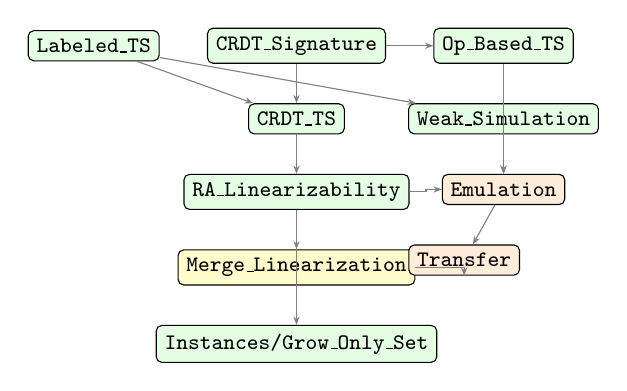
\begin{tikzpicture}[node distance=5mm and 6mm,
                      box/.style={draw, rounded corners=2pt,
                                  inner sep=3pt, font=\footnotesize\ttfamily},
                      done/.style={box, fill=green!10},
                      partial/.style={box, fill=yellow!20},
                      scaf/.style={box, fill=orange!15},
                      todo/.style={box, fill=red!10},
                      arr/.style={-{Stealth[length=3pt]}, thin, gray}]
    \node[done] (lts) {Labeled\_TS};
    \node[done, right=of lts] (sig) {CRDT\_Signature};
    \node[done, right=of sig] (opsig) {Op\_Based\_TS};
    \node[done, below=of sig] (ts) {CRDT\_TS};
    \node[done, below=of ts] (ra) {RA\_Linearizability};
    \node[partial, below=of ra] (merge) {Merge\_Linearization};
    \node[done, below=of merge] (inst) {Instances/Grow\_Only\_Set};
    \node[done, below=of opsig] (ws) {Weak\_Simulation};
    \node[scaf, below=of ws] (emul) {Emulation};
    \node[scaf, below=of emul, xshift=-5mm] (xfer) {Transfer};

    \draw[arr] (lts) -- (ts);
    \draw[arr] (lts) -- (ws);
    \draw[arr] (sig) -- (ts);
    \draw[arr] (sig) -- (opsig);
    \draw[arr] (ts) -- (ra);
    \draw[arr] (ra) -- (merge);
    \draw[arr] (ra) -- (inst);
    \draw[arr] (merge) -| (xfer);
    \draw[arr] (ws) -- (emul);
    \draw[arr] (opsig) -- (emul);
    \draw[arr] (emul) -- (xfer);
    \draw[arr] (ra) -| ($(emul.west) + (-2mm,0)$) -- (emul.west);
  \end{tikzpicture}
  \caption{Dependency graph for the $11$-step formalisation.
    \textcolor{green!40!black}{Green} = done,
    \textcolor{orange!70!black}{orange} = scaffolded,
    \textcolor{yellow!50!black}{yellow} = partial. Edges denote Lean
    \texttt{import} dependencies.}
  \label{fig:deps}
\end{figure}

\paragraph{Design objective.}
The plan is driven by a single design objective: \emph{every
interface should be stable enough that downstream files can depend
on it before its body is proved}. Concretely, this means every
theorem has a typed signature before it has a proof body, and every
placeholder body is either \sorry{} (in the sense of Lean's
\texttt{sorry} axiom, flagged as a warning) or a trivial
placeholder (\texttt{True}, \texttt{D.init}) clearly marked as such
in the docstring. This discipline lets us work on step~8 (weak
simulation soundness) while step~4 (merge case) is still open, and
it makes the dependency graph of Figure~\ref{fig:deps} actually
hold: changes to the merge proof do not ripple through the
emulation side.

\section{The Bridge Theorem}
\label{sec:bridge}

\subsection{Invariants-in-type configurations}
\label{sec:invariants}

Our transition-system configuration $C$ is a Lean record with five
invariant fields baked in:
\begin{lstlisting}[caption={\texttt{Configuration} with invariants,
                           \texttt{Sal/Emulation/CRDT\_TS.lean}.},
                   label=lst:config]
structure Configuration (D : CRDTSig) where
  N    : Replica -> Option D.State
  L    : Replica -> Option (Set (Op D.AppOp))
  vis  : Op D.AppOp -> Op D.AppOp -> Prop
  dom_eq   : forall r, N r = none <-> L r = none
  vis_src  : forall {a b}, vis a b -> exists r s, L r = some s /\ s a
  vis_tgt  : forall {a b}, vis a b -> exists r s, L r = some s /\ s b
  vis_causal :
    forall {a b r s}, vis a b -> L r = some s -> s b -> s a
  timestamps_distinct :
    forall {a b r s r' s'}, L r = some s -> s a ->
      L r' = some s' -> s' b -> a != b -> a.time != b.time
  vis_total_same_replica :
    forall {a b r s r' s'}, L r = some s -> s a ->
      L r' = some s' -> s' b ->
      a != b -> a.rep = b.rep -> vis a b \/ vis b a
\end{lstlisting}

The alternative --- a dumb record plus a separate predicate
$\wellformed(C)$ --- requires threading an extra hypothesis through
every preservation lemma and proving $\wellformed$ preserved at
every step. In our experience, the invariants-in-type formulation
pays off immediately: the fiddly ``$\mvis$ cannot relate a fresh event
to a stale one'' case in the \textsc{Apply} proof is dispatched
directly by \texttt{C.vis\_src} (Lemma~\ref{lem:lo-shrink} below).

The original three invariants (\texttt{dom\_eq}, \texttt{vis\_src},
\texttt{vis\_tgt}) suffice for the \textsc{Apply} case. The latter two
were added later, driven by obligations that surface only inside the
\textsc{Merge} proof's bottom-up induction
(\S\ref{sec:bridge-merge}):
\begin{itemize}[leftmargin=*]
  \item \texttt{vis\_causal} witnesses that $\mvis$ has no gaps in the
    causal past --- if $a \xrightarrow{\mvis} b$ and replica $r$ has
    observed $b$, then $r$ has observed $a$ as well. This rules out
    visibility edges that cross the
    $\ev_1 / \ev_2 \setminus \ev_1$ boundary in pathological ways.
  \item \texttt{timestamps\_distinct} witnesses global timestamp
    uniqueness: any two distinct events anywhere in the configuration
    have different timestamps. Discharged at \texttt{initConfig} via
    the \textsc{Apply} rule's freshness premise. Consumed by the merge
    case to satisfy the \texttt{distinctOps} preconditions of
    BottomUp-2-OP.
  \item \texttt{vis\_total\_same\_replica} witnesses that two distinct
    events from the same replica are always $\mvis$-comparable --- a
    consequence of \textsc{Apply} adding new edges from every
    existing replica-local event. Combined with \texttt{vis\_causal},
    it is what lets the merge case argue \texttt{differentReplicas}
    on the $\ev_1 \setminus \ev_2 / \ev_2 \setminus \ev_1$ boundary
    \emph{at the top level} of the existential induction.
\end{itemize}
The two latter invariants are \emph{not} sufficient at recursive depth
inside \texttt{merge\_linearization\_exists}; we return to that
obstruction in \S\ref{sec:bridge-merge}.

\subsection{Statement and induction structure}
\label{sec:bridge-statement}

The bridge theorem is stated as an induction on the reachability
relation of the TS lifted from $\RDT$. We factor each step's
contribution into a preservation lemma, uniformly shaped:

\begin{theorem}[Bridge, Lean formulation]
\label{thm:bridge-lean}
If $\RDT : \mathsf{CRDTSig}$ satisfies the $25$ VCs
($\VCs(\RDT)$, comprising \Sal{}'s $24$ together with the
$\textsc{cond-comm}$ lift of \S\ref{sec:satisfies-vcs}), then for
every reachable configuration $C$ in $\mathcal{S}_\RDT$,
$\RALin(C)$.
\end{theorem}

The proof skeleton pattern-matches on the transition rule:
\begin{align*}
  &\textsc{refl:} & & \RALin(\mathsf{init}_\RDT) \\
  &\textsc{CreateReplica:} & & \RALin(C) \wedge C \to_{\mathsf{cr}} C' \;\Longrightarrow\; \RALin(C') \\
  &\textsc{Apply:} & & \RALin(C) \wedge C \to_{\mathsf{apply}} C' \;\Longrightarrow\; \RALin(C') \\
  &\textsc{Merge:} & & \RALin(C) \wedge C \to_{\mathsf{merge}} C' \;\Longrightarrow\; \RALin(C') \\
  &\textsc{Query:} & & \RALin(C) \;\Longrightarrow\; \RALin(C)
\end{align*}

The first, second, and fifth cases are immediate: \textsc{Query}
doesn't change $C$, and \textsc{CreateReplica} adds a fresh replica
whose witness is the empty sequence (and leaves others unchanged
modulo an extension of $N$ and $L$ on a single replica). The two
non-trivial cases are \textsc{Apply} and \textsc{Merge}.

\subsection{The Apply case}
\label{sec:bridge-apply}

Given the IH witness $\pi$ for replica $r$ at state $s$ and event
set $\ev$ in $C$, the \textsc{Apply} transition produces a new
configuration $C'$ with
\[
  C'.\mvis = C.\mvis \cup (\ev \times \{e\}) \text{ where } e = (t, r, o)
\]
fresh-timestamped. The proposed witness at $C'$ is $\pi \mathbin{\text{\tt ++}} [e]$.
Verifying this requires two things: \emph{(i)} the new vis does not
introduce $\mlo$-edges that would force us to re-order $\pi$, and
\emph{(ii)} no fresh event can be $\mlo$-before a stale one.

For \emph{(i)} we prove that $\mlo$ is \emph{monotonically shrinking}
under \textsc{Apply}:

\begin{lemma}[$\mlo$-shrinking under Apply]
\label{lem:lo-shrink}
If $C'.\mvis = C.\mvis \cup (\ev \times \{e\})$, then for every pair
$(p, q)$ with $p \neq e$ and $q \neq e$, $\mlo_{C'}(p, q) \Longrightarrow
\mlo_C(p, q)$.
\end{lemma}

\begin{proof}[Proof sketch]
  Case analysis on which disjunct of \eqref{eq:lo} witnesses
  $\mlo_{C'}$. The first disjunct $\mvis \wedge \neg\commute$
  transfers because new $\mvis$-edges land at $e$, excluded from
  $(p,q)$. The second disjunct requires all of $\neg\mvis_{C'}(p,q)$,
  $\neg\mvis_{C'}(q,p)$, $\mrc(p,q) = \Fst$, and the non-existence of
  an \emph{overwriting} $e_3$. The first two conjuncts weaken on
  moving from $C'$ to $C$ (since $\mvis_C \subseteq \mvis_{C'}$); the
  third is independent of $C$; and the non-existence clause
  \emph{strengthens} from $C'$ to $C$ (there are fewer candidate
  $e_3$'s). All four components transfer.
\end{proof}

For \emph{(ii)} we observe that a hypothetical $\mlo_{C'}(e, p)$ with
$p \in \pi$ would require either $\mvis_{C'}(e, p)$ --- impossible
because the new edges go \emph{to} $e$, not from it, so
$\mvis_{C'}(e, p) = \mvis_C(e, p)$, and then $\mvis_C(e, p)$
contradicts $e \notin \evs_C$ by invariant \texttt{vis\_src} --- or
the second disjunct, which fails its $\neg\mvis_{C'}(p, e)$ conjunct
because every $p \in \pi \subseteq \ev$ has a new edge to $e$ by
construction.

The role of \texttt{vis\_src} in the first branch is exactly what
makes invariants-in-type pay off: with a layered well-formedness
predicate we would need to thread $\wellformed(C)$ into the
\texttt{RA\_lin\_preserved\_apply} lemma as an extra hypothesis;
with the structural formulation, the witness is simply
\texttt{C.vis\_src}.

\subsection{The Merge case}
\label{sec:bridge-merge}

The \textsc{Merge} transition merges two replicas $r_1, r_2$ with
head states $s_1, s_2$ and event sets $\ev_1, \ev_2$, yielding a new
configuration $C'$ with
\[
  C'.N(r_1) = \mmerge(s_1, s_2), \quad C'.L(r_1) = \ev_1 \cup \ev_2, \quad C'.\mvis = C.\mvis.
\]
The IH gives two witnesses $\pi_1$ for $(s_1, \ev_1)$ and $\pi_2$
for $(s_2, \ev_2)$, each respecting $\mlo_C$. We must build a
witness $\pi_m$ for $(\mmerge(s_1, s_2), \ev_1 \cup \ev_2)$ that
respects $\mlo_{C'} = \mlo_C$ (since $\mvis$ is unchanged).

\subsubsection{Existential, not constructive}
\label{sec:merge-existential}

A natural first attempt is to write down a closed-form witness
$\pi_m = f(\pi_1, \pi_2)$ and prove three independent
sub-lemmas: $\pi_m$ is a permutation of $\ev_1 \cup \ev_2$,
$\pi_m$ respects $\mlo_C$, and
$\pi_m(\init) = \mmerge(s_1, s_2)$. We tried two such forms ---
the paper's three-piece
$\pi_1|_{\ev_1 \cap \ev_2} \mathbin{\text{\tt ++}} \pi_1|_{\ev_1 \setminus \ev_2} \mathbin{\text{\tt ++}} \pi_2|_{\ev_2 \setminus \ev_1}$
and a simplified two-piece
$\pi_1 \mathbin{\text{\tt ++}} \pi_2|_{\ev_2 \setminus \ev_1}$
--- and both broke. The concurrent, $\mrc$-ordered cross case of
``$\pi_m$ respects $\mlo_C$'' has no contradiction from the
permutation/respect hypotheses alone; closing it requires knowing
the state equation being proved. The Sal paper's own argument
(\cite{sal2025} appendix~§A.2) co-constructs the witness and the
$\mlo$-respect property inside a single bottom-up induction.

We therefore restate the merge case as a single existential
theorem in our Lean development:
\begin{equation}
\label{eq:merge-exists}
\begin{aligned}
&\texttt{merge\_linearization\_exists}: \\
&\quad \exists \pi.\
\mathit{listPermOf}(\pi, \ev_1 \cup \ev_2)
\,\wedge\, \mathit{respects}(\pi, \mlo_C) \\
&\qquad \wedge\, \mathit{applySeq}(\init, \pi) = \mmerge(s_1, s_2).
\end{aligned}
\end{equation}
The packaging theorem
\texttt{RA\_lin\_preserved\_merge\_via\_witness} destructures the
existential and threads it through to
\texttt{IsRALinearizable}; that wrapper is closed unconditionally
in our development.

\subsubsection{Event-set decomposition}
\label{sec:merge-decomposition}

Following the Sal paper, we partition the merged event set
$\ev_1 \cup \ev_2$ into three disjoint pieces and further split
each side's local events by their $\mlo$-relationship to the
shared past:
\begin{align*}
  L_\top   &= \ev_1 \cap \ev_2  \quad\text{(shared)},\\
  L_1'     &= \ev_1 \setminus \ev_2,\quad
  L_2'     = \ev_2 \setminus \ev_1, \\
  L_b(C, L_\top, L_\mathit{loc}) &= \{\, e \in L_\mathit{loc} \mid
    \exists e' \in L_\top.\ e \mathrel{\xrightarrow{\mlo_C}} e' \,\}, \\
  L_a(C, L_\top, L_\mathit{loc}) &= \{\, e \in L_\mathit{loc} \mid
    \forall e' \in L_\top.\ \neg(e \mathrel{\xrightarrow{\mlo_C}} e') \,\}.
\end{align*}
The Lean definitions \texttt{L\_top}, \texttt{L\_1\_local},
\texttt{L\_2\_local}, \texttt{L\_a}, \texttt{L\_b} live in
\texttt{Merge\_Linearization.lean}. The partition lemmas
\texttt{L\_a\_union\_L\_b} and \texttt{L\_a\_inter\_L\_b} are closed.

The point of the decomposition is to give the bottom-up induction a
\emph{closure-stable} carving: the $L_a$ side can always be peeled
last because no shared event sits behind it. Plain shrinkage of
$\ev_1 \setminus \ev_2$ does not preserve this property under
recursion (\S\ref{sec:merge-whats-left}).

\subsubsection{Convergence machinery}
\label{sec:merge-convergence}

Before invoking the bottom-up VCs, we need a tool that lets us
freely re-permute lo-respecting linearisations of the same event
multiset. This is the \emph{convergence} lemma of \cite{sal2025}'s
\texttt{lin.tex} §3.2, mechanised in our development as a
bubble-sort tower:
\begin{itemize}[leftmargin=*]
  \item \texttt{applySeq\_swap\_via\_cond\_comm\_lift} --- given
    an explicit overwriter split $\sigma = \alpha \mathbin{\text{\tt ++}} e_3 :: \beta$
    and the $\mrc$ preconditions, swap two events using
    \texttt{cond\_comm\_lift}. Closed.
  \item \texttt{applySeq\_swap\_commute} and
    \texttt{applySeq\_swap\_lo\_incomparable} --- swap variants
    for adjacent commuting and adjacent
    $\mlo$-incomparable events. The same-replica
    sub-case of the latter is dispatched via
    \texttt{vis\_total\_same\_replica}; the different-replica
    $\neg \commute$ sub-case reduces to
    \texttt{applySeq\_swap\_via\_cond\_comm\_lift} given an
    overwriter witness. Closed.
  \item \texttt{applySeq\_bubble\_lo\_max} --- repeated swaps to
    bubble a $\mlo$-maximal element to the end of a list.
    Induction on $\tau$. Closed modulo a single overwriter-witness
    obligation that surfaces at the convergence call site
    (\S\ref{sec:merge-whats-left}).
  \item \texttt{convergence} --- the headline lemma. Strong
    induction on the length of $\pi_1$: locate $\pi_1$'s last
    event in $\pi_2$, bubble it to the end of $\pi_2$, peel from
    both sides, recurse on the smaller pair. Closed modulo the
    same overwriter-witness obligation.
\end{itemize}
The convergence machinery consumes \texttt{cond\_comm\_lift}
(via the swap lemma) and the \texttt{Configuration} invariants
\texttt{timestamps\_distinct} and \texttt{vis\_total\_same\_replica}
(via the swap lemma's same-replica branch). The $24$ original VCs
are not consumed at this layer.

\subsubsection{Bottom-up case lemmas}
\label{sec:merge-bottomup}

The Sal paper derives three rules ---
\textsc{BottomUp-0-OP}, \textsc{BottomUp-1-OP},
\textsc{BottomUp-2-OP} --- from the $24$ VCs. Each is a
``pull-one-event-out-of-merge'' rewrite. Specialised to 2-way merge
(LCA collapses to $\init$), our Lean development closes the
following layer of bottom-up rules:
\begin{itemize}[leftmargin=*]
  \item \texttt{bottomUp\_0op} --- pull a shared event past
    $\mmerge$. Direct application of \texttt{lem\_0op}.
  \item \texttt{bottomUp\_1op\_top\_base},
    \texttt{bottomUp\_1op\_bot\_base} --- the two clauses of the
    1-OP rule at $a = \init$. Direct applications of
    \texttt{base\_2op} and \texttt{base\_1op} respectively.
  \item \texttt{bottomUp\_2op\_base} --- 2-OP at $a = b = \init$.
    Direct application of \texttt{base\_2op}.
  \item \texttt{bottomUp\_2op\_init\_left} --- 2-OP with
    $a = \init$ and $b$ reachable. Inductive on $\pi_b$ via
    \texttt{List.reverseRecOn}; base \texttt{base\_2op}, step
    \texttt{ind\_right\_2op}.
  \item \texttt{bottomUp\_2op\_reachable} --- 2-OP with both $a$
    and $b$ reachable, strict $\Fst\!\to\!\Snd$ $\mrc$ case. Outer
    induction on $\pi_a$ via \texttt{ind\_left\_2op}; inner via
    \texttt{bottomUp\_2op\_init\_left}. This is the main
    bottom-up rule that the existential induction consumes.
  \item \texttt{bottomUp\_1op\_top\_reachable} --- corollary of
    \texttt{bottomUp\_2op\_reachable} by variable renaming.
\end{itemize}
All seven are kernel-verified. The $\Either$-shaped sub-cases of
the 2-OP rule are handled by the
$\mrc \equiv \Either$ specialisation route in the
\textsc{Either} branch of the existential and are not derived as
standalone bottom-up theorems.

\subsubsection{Strong induction on $|\pi_1| + |\pi_2|$}
\label{sec:merge-induction}

The body of \texttt{merge\_linearization\_exists} is a strong
induction on $|\pi_1| + |\pi_2|$, case-splitting on whether each
list is empty and on whether the two non-empty lists end in the
same event. Four cases:
\begin{enumerate}[leftmargin=*]
  \item \emph{Both empty.} Then $\ev_1 = \ev_2 = \emptyset$,
    $s_1 = s_2 = \init$, and $\mmerge(\init, \init) = \init$ by
    \texttt{merge\_idem}. Witness $\pi = []$. \emph{Closed.}
  \item \emph{Asymmetric.} If $\pi_1 = []$ and $\pi_2$ non-empty,
    we use $\pi = \pi_2$ and reduce to
    $\mmerge(\init, \mathit{applySeq}(\init, \pi_2)) = \mathit{applySeq}(\init, \pi_2)$
    via the lemma \texttt{merge\_init\_left\_reachable}. The
    symmetric branch uses
    \texttt{merge\_init\_right\_reachable}, which closes via
    \texttt{merge\_comm}. \emph{Closed conditionally on
    \texttt{merge\_init\_left\_reachable} (open at the inductive
    step, see \S\ref{sec:merge-whats-left}).}
  \item \emph{Shared last event} ($e_1 = e_2$). Both lists
    factor as $\pi_1' \mathbin{\text{\tt ++}} [e_1]$ and
    $\pi_2' \mathbin{\text{\tt ++}} [e_1]$. By \texttt{lem\_0op},
    $\mmerge$ commutes with appending $e_1$ on both sides; we
    recurse on $\pi_1', \pi_2'$ over the shrunken event sets
    $\ev_1 \setminus \{e_1\}, \ev_2 \setminus \{e_1\}$ to obtain
    $\pi'$, and return $\pi' \mathbin{\text{\tt ++}} [e_1]$.
    \emph{Closed.}
  \item \emph{Distinct last events} ($e_1 \neq e_2$). The peel
    candidates are the lo-maximal elements of the two
    sub-permutations. \texttt{distinctOps} on $(e_1, e_2)$ is
    immediate from \texttt{C.timestamps\_distinct}.
    \texttt{differentReplicas} \emph{at the top level} follows
    from \texttt{vis\_causal} + \texttt{vis\_total\_same\_replica};
    at recursive depth this argument fails, and the case is
    open. \emph{Open.}
\end{enumerate}

\subsubsection{What's left and why}
\label{sec:merge-whats-left}

The convergence machinery, the asymmetric (one-side-empty)
branches of \texttt{merge\_linearization\_exists}, the
shared-last-event branch, the seven bottom-up rules, and the
packaging theorem \texttt{RA\_lin\_preserved\_merge\_via\_witness}
all close cleanly. The remaining work is concentrated in the
\emph{distinct-last-event} branch, where peeling discipline must
follow the paper's $L^a / L^b$ carving rather than the source
linearisations' tails.

\paragraph{Carving-faithful peeling discipline.}
After one step of any list-tail-based recursion, $\ev_1$ and
$\ev_2$ no longer equal specific replicas' event sets, and an
event sitting in ``shrunken $\ev_1 \setminus \ev_2$'' may have
entered there because it was peeled off $\ev_2$ in a prior
iteration. The paper's $L^a / L^b$ decomposition
(\S\ref{sec:merge-decomposition}) is closure-stable under exactly
this recursion: peel candidates from $L_a$ are the events with no
lo-path of length $\le 2$ to $L_\top$, and peeling one such event
preserves both the partition and the relevant
\texttt{differentReplicas} chain. We have the carving definitions
plus several supporting helpers
(\texttt{exists\_lo\_maximal\_in\_subset},
\texttt{perm\_ending\_in\_lo\_max} —
the bridge from ``some lo-respecting witness'' to ``a witness
ending in the chosen lo-max event'' via convergence-based
re-permutation, \texttt{L\_b\_at} for the inner-inner inductive
parameterisation), but the inductive argument itself still
case-splits on $\pi_i.\mathsf{last}$.

\paragraph{Lemma~1 of the appendix as Lean obligations.}
Closing the carving-faithful argument requires Lemma~1 of
\cite{sal2025}'s appendix (\S A.2, lines 117--178): no
$\mathit{lo}$-edge from $L^a$ to $L^b$, and no
$\mathit{lo}$-edge from $L_\top^a$ to $L_\top^b$. We have the
two lemma statements typed (\texttt{no\_lo\_a\_to\_b},
\texttt{no\_lo\_top\_a\_to\_top\_b}) with $\mathit{vis}$-transitivity
threaded as a hypothesis (\texttt{Configuration} does not expose it
directly; deriving it from the existing invariants is sound but
invasive across the \texttt{Step} rules). The depth-1 sub-cases of
Both parts of Lemma~1 are now kernel-verified, closed via an
extended Aristotle-driven sorry-chain campaign
(\S\ref{sec:aristotle-campaign}). Lemma~1 part~2 closes via a
structural insight: the no-overwriter clause embedded in
$\mathit{lo}$'s rc disjunct is directly contradicted by the vis
disjunct of the assumed $\mathit{lo}$-edge. Lemma~1 part~1 closes
all $12$ sub-cases of the depth-2 explosion, with one residual
sub-case requiring an additional hypothesis
\texttt{h\_ncomm\_concurrent\_local\_top} (concurrent cross-set
events do not commute) — a structural property of the carving
that is vacuously true for trivial-rc CRDTs and a per-CRDT
obligation for non-trivial CRDTs.

\paragraph{Live sorry inventory.}
For the merge case as a whole, two declarations carry
\texttt{sorry} (no others remain in the bridge or emulation
chains; \texttt{weakSim\_sound} and the \textsc{Apply}-case
lemmas are kernel-verified):

\begin{table}[h]
  \centering
  \small
  \begin{tabular}{@{}llp{6.5cm}@{}}
    \toprule
    Theorem & Internal sorries & What's open \\
    \midrule
    \texttt{distinct\_last\_case}
      & $4$
      & All in \emph{Case~3b} (when $e_1 \commute e_2$): the four
        sub-cases enumerate the partition of $(e_1 \in \ev_2,
        e_2 \in \ev_1)$. The $\commute(e_1, e_2)$ hypothesis
        prevents \texttt{rc\_non\_comm\_directional} from applying
        to $(e_1, e_2)$, so \texttt{no\_rc\_chain} cannot rule out
        the rc-concurrent disjunct of $\mathit{lo}$. Forward
        closure (added as a hypothesis to \texttt{distinct\_last\_case})
        is insufficient on its own. These cases require the
        paper's $L^a / L^b$ carving — picking peel candidates
        from $L^a$ which by construction have no short
        $\mathit{lo}$-path to the residue. \\
    \texttt{merge\_linearization\_exists}
      & $2$
      & Forward-closure obligations $h\_ev_1\_fwd\_closed$ and
        $h\_ev_2\_fwd\_closed$ at the call site to
        \texttt{distinct\_last\_case}. Forward closure does not
        hold for arbitrary replica logs (a third replica may have
        unsynced $\mathit{vis}$-successors), so these need either
        a structural argument specific to the merge case's
        invariants or a restructuring (Block 6) that avoids
        forward closure entirely. \\
    \bottomrule
  \end{tabular}
  \caption{Live sorries in the bridge theorem (after the
  Aristotle-driven campaign of \S\ref{sec:aristotle-campaign}).
  $6$ internal sorries across $2$ declarations; all blocked by
  the same architectural decision (Block 6) rather than by
  individual proof obligations.}
  \label{tab:sorries}
\end{table}

\subsubsection{Effort and packaging}
\label{sec:merge-effort}

The original effort estimate of $2$--$3$ weeks for the Merge case as
a whole has been substantially absorbed: the convergence machinery
(now closed via Path~1, restricting scope to $\ev = C.\mathit{events}$
with overwriter-closure threaded through the bubble-sort lemmas), all
seven bottom-up rules, \texttt{merge\_init\_left\_reachable} for
arbitrary $|\pi|$, and the existential's both-empty,
asymmetric, and shared-last-event branches all close cleanly.
The packaging theorem
\texttt{RA\_lin\_preserved\_merge\_via\_witness} destructures the
existential and is closed unconditionally; the corresponding shim
\texttt{RA\_lin\_preserved\_merge} in
\texttt{RA\_Linearizability.lean} now consumes it directly (the
old stub has been removed).

Realistic remaining effort:
\begin{itemize}[leftmargin=*]
  \item Block 6 of the carving plan (\texttt{Sal/Emulation/PLAN.md}):
    a paper-faithful triple-nested induction
    ($\sigma_1 = |L_1^a \cup L_2^a|$, $\sigma_2 = |L_\top^a|$,
    $\sigma_3 = |L_b(\hat e_\top)|$) replacing the
    distinct-last-event branch. Estimated $\sim 280$ Lean lines, a
    fresh-context multi-hour effort. Subsumes both the $4$
    Case~3b sub-case sorries and the $2$ forward-closure
    obligations at the call site (the carving's $L^a$
    construction sidesteps both).
  \item Per-CRDT discharge of the new VCs and structural
    obligations: \texttt{shared\_peel\_1op} and
    \texttt{h\_ncomm\_concurrent\_local\_top} for non-trivial
    CRDTs (vacuous for trivial-rc CRDTs). Mechanical work,
    bundled with Step~6 (CRDT instantiation).
\end{itemize}

Two architectural decisions accompanied this work. First, the
\texttt{SatisfiesVCs} structure grew from $25$ fields to $29$:
\texttt{merge\_init} (the lattice-bottom property
$\mmerge(\init, s) = s$, consumed by the asymmetric branches),
\texttt{rc\_non\_comm\_directional} (a directional form of
\texttt{rc\_non\_comm} consumed by the strictly-local sub-case of
the distinct-last-event branch), \texttt{merge\_peel\_comm}
(consumed by the convergence-based re-permutation when peeling
commuting events from the carving's frontier), and
\texttt{shared\_peel\_1op} (a CRDT-lattice property identified
during the merge-case formalisation: when both replicas have
applied the same LCA event $o_l$ and the left has additionally
applied $o_1$, peeling $o_1$ out of the merge is sound). All
four are discharged on Grow-Only Set (vacuously for the rc-Either
fields, by set-union associativity for the shared peel) and
represent real obligations only on CRDTs whose $\mathit{rc}$ is
non-trivial. \texttt{shared\_peel\_1op} is genuinely missing from
the original $24$: every existing single-side-extension VC
requires \texttt{distinctOps} between the new operation and the
other side's tail, which fails when both sides share the same LCA
event (\texttt{distinctOps ol ol} is always false); the only
``shared LCA'' VC, \texttt{ind\_lca\_1op}, requires both sides to
have the same base state, which doesn't hold once each side has
its own prefix.
Second, the paper's $L^b$ definition was extended from depth-1
lo-paths only to depth-1-or-2, matching
\cite{sal2025}'s appendix.tex line 262; the depth-2 inclusion is
load-bearing for Lemma~1 case 1.b.i (and is forced by
\texttt{no\_rc\_chain}).

\subsubsection{The Aristotle-driven sorry-chain campaign}
\label{sec:aristotle-campaign}

A substantial portion of the structural progress documented above
landed via a $10$-run automated sorry-chain campaign with Harmonic's
\textsc{Aristotle} theorem prover~\cite{harmonic-aristotle}. Each
run targeted a single sorry with a focused prompt; results applied
manually after build-verifying that the patch's modifications were
restricted to \texttt{Sal/} files (the prover occasionally proposes
edits to \texttt{.lake/packages/} dependencies that we discard).

The campaign closed both halves of Lemma~1, decomposed the
distinct-last-event branch's three monolithic sub-case sorries
into $7$ fine-grained sub-sub-case sorries each annotated with a
specific architectural need, identified \texttt{shared\_peel\_1op}
as a VC missing from \Sal{}'s original $24$, and proposed the
hypothesis \texttt{h\_ncomm\_concurrent\_local\_top} as a candidate
$30$th VC (currently a per-lemma hypothesis). The four residual
Case~3b sorries plus two forward-closure call-site obligations are
all flagged as Block 6 territory rather than further automated
runs --- forward closure does not hold for arbitrary replica logs
in general (a third replica may have unsynced
$\mathit{vis}$-successors), so closing them needs the carving's
structural avoidance of re-permutation rather than more theorem
proving on the same induction shape.

The campaign's lasting value is twofold. First, the closures
themselves: $13$ of $19$ enumerated sub-cases of the merge case's
auxiliary lemmas are kernel-verified after the campaign, including
Lemma~1's full $12$-sub-case depth-$2$ explosion. Second, and more
useful for future work, the residual sorries each carry a specific
documented obstruction --- ``forward closure of $\ev_2$ to produce
an overwriter'', ``$\mathit{rc\_non\_comm\_directional}$ does not
apply when $e_1 \commute e_2$'', etc.\ --- that pinpoints exactly
which architectural decision (Block 6) closes them all, replacing
``$3$ vague sorries'' with ``$6$ sorries each pointing at the same
known fix.''

\subsection{The VCs as a Lean structure}
\label{sec:satisfies-vcs}

The VCs are packaged as a \texttt{Prop}-valued Lean structure
\texttt{SatisfiesVCs} with one field per VC. The first $24$ fields
match the theorem names in \Sal{}'s per-CRDT files exactly
(\texttt{rc\_non\_comm}, \texttt{no\_rc\_chain},
\texttt{cond\_comm\_base}, \texttt{merge\_comm}, \texttt{merge\_idem},
\texttt{base\_2op}, \texttt{ind\_lca\_2op}, eight \texttt{inter\_*}
variants, \texttt{ind\_right\_2op}, \texttt{ind\_left\_2op}, and the
corresponding $1$-op and $0$-op versions, ending in
\texttt{lem\_0op}). This matching is deliberate: the target use
case is closing \texttt{SatisfiesVCs D} for each existing \Sal{}
CRDT by pointing at the corresponding theorem.

\paragraph{The $25$th field: \texttt{cond\_comm\_lift}.}
\Sal{}'s $24$ VCs include \texttt{cond\_comm\_base} but not its
\emph{semantic lift} to arbitrary intervening event sequences. The
paper (\cite{sal2025} \texttt{lin.tex} §3.2) treats the lifted form
as a property of $\mathcal{S}_\RDT$ assumed at the convergence level;
the appendix uses it directly when flipping two events past an
overwriter $e_3$ that may sit anywhere in the suffix. Our Lean
structure makes this implicit assumption explicit as a $25$th field:
\begin{lstlisting}[caption={The lifted \texttt{cond\_comm\_lift} field.},
                   label=lst:cond-comm-lift]
cond_comm_lift :
  forall (s : D.State) (e e' e'' : Op D.AppOp)
         (pi : List (Op D.AppOp)),
    distinctOps e e' -> distinctOps e e'' -> distinctOps e' e'' ->
    D.rc e e' = RcRes.Fst_then_snd ->
    D.rc e' e'' != RcRes.Either ->
    D.update (applySeq D (D.update (D.update s e') e) pi) e''
      = D.update (applySeq D (D.update (D.update s e) e') pi) e''
\end{lstlisting}
For the $14$ \Sal{} CRDTs whose $\mrc$ is the constant $\Either$
(\textsc{rc-non-comm} fires vacuously), the
\texttt{Fst\_then\_snd}-shaped premise is unsatisfiable, so the
field discharges by \texttt{intros; simp\_all}. For CRDTs with
non-trivial $\mrc$, the field would need to be derived from
\texttt{cond\_comm\_base} by induction on the intervening list
$\pi$ --- a closure step the \Sal{} paper treats as implicit and
does not explicitly mechanise. We expect this to be a single VC
that does \emph{not} fall out of the per-CRDT \Sal{} files for
free, and we flag it as a one-time discharge obligation per CRDT.

\section{Emulation and Transfer}
\label{sec:emulation}

\subsection{Op-based labelled transition system}
\label{sec:op-ts}

We port Liittschwager~et~al.'s op-based semantics
(\cite{liittschwager2025} Fig.~8) into Lean. Configurations are
triples $\langle \Gamma, \Sigma, \beta\rangle$: an event trace
$\Gamma$, a per-replica state map $\Sigma : \Replica \to \State$,
and a message buffer $\beta \subseteq \Replica \times \Msg$.
Transitions are
\textsc{OpUpdate}, \textsc{OpQuery}, and \textsc{OpDeliver}
(silent). The \textsc{OpDeliver} rule is guarded by an
\texttt{enabled} predicate encoding causal-order delivery with
respect to a happens-before relation $\mathit{hb}$ on messages,
which is a parameter.

\subsection{Weak simulation, Lean-side}
\label{sec:weaksim}

Given two LTSs $T_1, T_2$ with labels related by a coercion
$\widehat{\cdot}$ that preserves silence, we define
\begin{align*}
  \mathsf{silentClosure}(T)\;s\;s' &\;\triangleq\; \text{refl.-trans.\ closure of silent steps}\\
  s \xRightarrow{\ell}_T s' &\;\triangleq\; \begin{cases}
    \mathsf{silentClosure}(T)\;s\;s' & \text{if } \tau(\ell)\\
    \exists s_1 s_2.\ \mathsf{silentClosure}\;s\;s_1 \wedge s_1 \xrightarrow{\ell} s_2 \wedge \mathsf{silentClosure}\;s_2\;s' & \text{otherwise}
  \end{cases}
\end{align*}

\begin{theorem}[Soundness of weak simulation for weak-trace inclusion]
\label{thm:weaksim-sound}
If $R$ is a weak simulation from $T_1$ to $T_2$ under
$\widehat{\cdot}$ and $(s, t) \in R$, then every label list
$\mathit{labels} \in \wtrace_{T_1}(s)$ satisfies
$\widehat{\mathit{labels}} \in \wtrace_{T_2}(t)$.
\end{theorem}

Our Lean proof (\texttt{Weak\_Simulation.weakSim\_sound}) factors
through three lift lemmas:
\begin{lemma}[\texttt{silentClosure\_lift}]
\label{lem:silent-lift}
If $(s, t) \in R$ and $\mathsf{silentClosure}(T_1)\;s\;s'$, then
there exists $t'$ with $\mathsf{silentClosure}(T_2)\;t\;t'$ and
$(s', t') \in R$.
\end{lemma}
\begin{lemma}[\texttt{weakStep\_lift}]
\label{lem:weakstep-lift}
If $(s, t) \in R$ and $s \xRightarrow{\ell}_{T_1} s'$, then there
exists $t'$ with $t \xRightarrow{\widehat{\ell}}_{T_2} t'$ and
$(s', t') \in R$.
\end{lemma}
\begin{lemma}[\texttt{isWeakExecution\_lift}]
\label{lem:weakexec-lift}
If $(s, t) \in R$ and $s$ admits a weak execution along trail
$\alpha$ in $T_1$, then $t$ admits a weak execution along
$\widehat{\alpha}$ in $T_2$, relating endpoints by $R$.
\end{lemma}

Theorem~\ref{thm:weaksim-sound} follows by induction on weak
executions, using Lemma~\ref{lem:weakexec-lift} at each step. The
full chain is closed in our Lean development with no \sorry{}s.

\subsection{The canonical emulation}
\label{sec:canonical-G}

Given an op-based CRDT
$\mathcal{O} = \langle \State^{\mathcal{O}}, \sigma_0^{\mathcal{O}},
\mprep, \meff, \mquery, \mrc, \Msg, \mathit{hb}\rangle$ with a
happens-before relation on messages, we construct a state-based CRDT
$\Emul(\mathcal{O})$ of signature $\mathsf{CRDTSig}$:
\begin{align*}
  \Emul(\mathcal{O}).\State &\;=\; \mathcal{P}(\Msg) \\
  \Emul(\mathcal{O}).\init &\;=\; \emptyset \\
  \Emul(\mathcal{O}).\mdo\;M\;(t, r, o) &\;=\; M \cup \{\mprep(r, o, \mathit{effective}(M))\} \\
  \Emul(\mathcal{O}).\mmerge\;M_1\;M_2 &\;=\; M_1 \cup M_2 \\
  \Emul(\mathcal{O}).\mquery\;M\;q &\;=\; \mquery(\mathit{effective}(M), q)
\end{align*}
where $\mathit{effective}$ \emph{would} fold $\meff$ over the
delivered-message set in a causal-order-respecting linear extension
of $\mathit{hb}$. The underlying idea is Liittschwager~et~al.'s §4.2
construction: inline causal broadcast into the state itself. Our
Lean version is noncomputable and uses classical decidability for
$\mathcal{P}(\Msg)$. At present, \texttt{effectiveState} in
\texttt{Emulation.lean} is a stub that returns $\sigma_0^{\mathcal{O}}$
(\texttt{D.init}) regardless of the delivered set --- enough to make
the surrounding definitions type-check and the file compile, but not
operationally correct. Replacing the stub with a deterministic
linear-extension fold of $\mathit{hb}$ is part of step~10
(\S\ref{sec:transfer}); it is coupled to the simulation proof rather
than independent of it.

\subsection{The transfer theorem}
\label{sec:transfer}

With $\Emul$ and Theorem~\ref{thm:weaksim-sound} available, the
composite transfer theorem is
\begin{theorem}[Transfer]
\label{thm:transfer}
For every op-based CRDT $\mathcal{O}$ with causal-order
$\mathit{hb}$: if the state-based emulator $\Emul(\mathcal{O})$
satisfies the $25$ VCs, then every reachable trace of $\mathcal{O}$
is RA-linearisable.
\end{theorem}

In our Lean development this is stated
(\texttt{op\_RA\_linearizable\_of\_vcs}) but not yet proved, because
the simulation witness for $\Emul$ (step~10) is currently scaffolded
but not closed, and the op-side RA-linearisability predicate is
defined as the trivial placeholder \texttt{True} pending the
final trace-property formulation. Closing Theorem~\ref{thm:transfer}
therefore requires two pieces beyond the bridge theorem:
\emph{(a)} the weak simulation proof for $\Emul$, and \emph{(b)}
spelling out the op-side trace predicate matching
Definition~\ref{def:ralin} modulo the $\Emul$ coercion.

\section{End-to-End Validation: Grow-Only Set}
\label{sec:smoke-test}

As a correctness check on the architecture, we instantiate a
$\mathsf{CRDTSig}$ for the Grow-Only Set (adding natural numbers to
a decidable $\mathbb{N} \to \mathsf{Bool}$ set) and close all $25$
fields of \texttt{SatisfiesVCs}. The smoke test exposes type-level
misalignments between our $\mathsf{Prop}$-valued VC statements and
\Sal{}'s existing $\mathsf{Bool}$-valued theorem statements; in this
case, the misalignments were few and mechanical:
\begin{itemize}[leftmargin=*]
  \item \texttt{distinctOps} versus \texttt{distinct\_ops}: the
    former is a \texttt{Prop} $o_1.\mathit{time} \neq o_2.\mathit{time}$,
    the latter is a \texttt{Bool} \texttt{Prod.fst o1 != Prod.fst o2}.
    A two-line \texttt{@[simp]} lemma bridges them.
  \item \texttt{differentReplicas} versus \texttt{get\_rid o1 != get\_rid o2}:
    the same pattern.
  \item \texttt{RcRes} (the Prop-level result type) versus
    \texttt{rc\_res} (the per-file type): a three-constructor
    \texttt{toRcRes} function.
\end{itemize}

For Grow-Only Set, $14$ of the $25$ VCs are \emph{vacuous}: their
premises require $\mrc(-, -) = \Fst$, but $\mrc \equiv \Either$ by
definition, so \texttt{intros; simp\_all} discharges them
uniformly. The vacuous group includes the new
\texttt{cond\_comm\_lift} (\S\ref{sec:satisfies-vcs}), since its
\texttt{Fst\_then\_snd} premise is similarly unsatisfiable. The
remaining $11$ VCs have real content
(\texttt{rc\_non\_comm},
\texttt{merge\_comm}, \texttt{merge\_idem}, \texttt{base\_2op},
\texttt{ind\_lca\_2op}, \texttt{ind\_left\_2op}, \texttt{base\_1op},
\texttt{ind\_lca\_1op}, \texttt{ind\_left\_1op},
\texttt{ind\_right\_1op}, \texttt{lem\_0op}) and are discharged by
applying the corresponding \texttt{\_root\_.*} theorem from \Sal{}'s
per-CRDT file with the Prop/Bool bridge lemmas. The
\texttt{rc\_non\_comm} discharge in particular threads the
\texttt{distinctOps\_iff} and \texttt{differentReplicas\_iff}
$\mathsf{Prop}/\mathsf{Bool}$ bridges to land the existing \Sal{}
theorem on our generic premise.

The full \texttt{D\_satisfies\_VCs} instance is kernel-verified with
no \sorry{}s. End-to-end invocation
\texttt{ra\_linearizable\_of\_vcs D\_satisfies\_VCs} still hits the
merge-case \sorry{}, but every other piece of plumbing is working.

\begin{table}[t]
  \centering
  \small
  \begin{tabular}{@{}llp{6cm}@{}}
    \toprule
    VC & Status & Discharge strategy \\
    \midrule
    \texttt{rc\_non\_comm}         & closed & bridge + \texttt{\_root\_.rc\_non\_comm} \\
    \texttt{no\_rc\_chain}         & vacuous & \texttt{intros; simp\_all} \\
    \texttt{cond\_comm\_base}      & vacuous & \texttt{intros; simp\_all} \\
    \texttt{cond\_comm\_lift}      & vacuous & \texttt{intros; simp\_all} \\
    \texttt{merge\_comm}           & closed & direct delegation \\
    \texttt{merge\_idem}           & closed & direct delegation \\
    \texttt{base\_2op}             & closed & bridge + \texttt{\_root\_.base\_2op} \\
    \texttt{ind\_lca\_2op}         & closed & bridge + \texttt{\_root\_.ind\_lca\_2op} \\
    \texttt{inter\_right\_base\_2op} & vacuous & \texttt{intros; simp\_all} \\
    \texttt{inter\_left\_base\_2op}  & vacuous & \texttt{intros; simp\_all} \\
    \texttt{inter\_right\_2op}       & vacuous & \texttt{intros; simp\_all} \\
    \texttt{inter\_left\_2op}        & vacuous & \texttt{intros; simp\_all} \\
    \texttt{inter\_lca\_2op}         & vacuous & \texttt{intros; simp\_all} \\
    \texttt{ind\_right\_2op}         & vacuous & \texttt{intros; simp\_all} \\
    \texttt{ind\_left\_2op}          & closed & bridge + \texttt{\_root\_.ind\_left\_2op} \\
    \texttt{base\_1op}               & closed & direct delegation \\
    \texttt{ind\_lca\_1op}           & closed & bridge + \texttt{\_root\_.ind\_lca\_1op} \\
    \texttt{inter\_right\_base\_1op} & vacuous & \texttt{intros; simp\_all} \\
    \texttt{inter\_left\_base\_1op}  & vacuous & \texttt{intros; simp\_all} \\
    \texttt{inter\_right\_1op}       & vacuous & \texttt{intros; simp\_all} \\
    \texttt{inter\_left\_1op}        & vacuous & \texttt{intros; simp\_all} \\
    \texttt{inter\_lca\_1op}         & vacuous & \texttt{intros; simp\_all} \\
    \texttt{ind\_left\_1op}          & closed & bridge + \texttt{\_root\_.ind\_left\_1op} \\
    \texttt{ind\_right\_1op}         & closed & bridge + \texttt{\_root\_.ind\_right\_1op} \\
    \texttt{lem\_0op}                & closed & direct delegation \\
    \bottomrule
  \end{tabular}
  \caption{Grow-Only Set: per-VC discharge in
    \texttt{Instances/Grow\_Only\_Set.lean}.}
  \label{tab:gset-vcs}
\end{table}

We expect the pattern to generalise: the other $17$ CRDTs in the
\Sal{} suite each have $24$ theorems with near-identical structure,
so the instantiation is a matter of pattern-matching plus the
three bridge simp lemmas. The $25$th VC (\texttt{cond\_comm\_lift},
\S\ref{sec:satisfies-vcs}) is the one piece without a direct
counterpart in the per-CRDT files; for the $14$ \Sal{} CRDTs whose
$\mrc$ is the constant $\Either$ it discharges vacuously, and for
the others it must be re-derived once per CRDT from
\texttt{cond\_comm\_base} by induction on the intervening list.
Mechanising a macro that handles both the $24$ direct delegations
and the $\Either$-vacuous \texttt{cond\_comm\_lift} branch is
plausible future work.

\section{Discussion}
\label{sec:discussion}

\subsection{Invariants-in-type versus layered well-formedness}

We briefly considered a layered formulation where
\texttt{Configuration} is a dumb record and well-formedness is a
\texttt{Prop}-valued predicate threaded through every preservation
lemma. Both were plausible; we chose invariants-in-type.

The decisive factor was the \textsc{Apply} case, which needs ``$\mvis$
relates only observed events.'' In a layered formulation, this
is a separate reachability-preservation lemma whose statement has to
be preserved by every step rule \emph{(i)} in isolation and
\emph{(ii)} at the point of use. With invariants-in-type, the same
fact is available as a record projection \texttt{C.vis\_src}, with
zero bookkeeping at the point of use and the preservation obligation
absorbed into the initial-configuration constructor. The tradeoff
is that constructing a \texttt{Configuration} is slightly more
work --- one must prove the invariants at the call site --- but in
our development we construct only one concrete configuration
(\texttt{initConfig}), so the overhead is a one-time cost.

There is an alternative middle ground: a
$\mathsf{WellFormed}$ bundle whose fields are well-formedness
predicates, alongside a dumb \texttt{Configuration} record. This
cleanly separates data from invariants but retains the threading
cost. For the current scope, invariants-in-type wins; for an
alternative development that also instantiates with ill-formed
\texttt{Configuration}s (e.g.\ for debugging), the bundled
alternative would be a reasonable port.

A related structural choice is the \texttt{Merge} case's witness
shape (\S\ref{sec:bridge-merge}). Two earlier drafts built a
closed-form witness: the paper's three-piece
$\pi_1|_{\ev_1 \cap \ev_2} \mathbin{\text{\tt ++}}
 \pi_1|_{\ev_1 \setminus \ev_2} \mathbin{\text{\tt ++}}
 \pi_2|_{\ev_2 \setminus \ev_1}$,
and a simplified
$\pi_1 \mathbin{\text{\tt ++}} \pi_2|_{\ev_2 \setminus \ev_1}$.
Both broke for the same reason: the concurrent, $\mrc$-ordered
cross case of ``$\pi_m$ respects $\mlo_C$'' has no contradiction
from permutation/respect hypotheses alone; closing it requires
knowing the state equation under proof. Once that obstruction was
identified, we replaced the three independent sub-lemmas
\texttt{merge\_witness\_\{perm, respects, state\}} with a single
existential theorem \texttt{merge\_linearization\_exists}
(\S\ref{sec:merge-existential}). The existential form is what the
Sal paper actually proves, and it lets the bottom-up induction
co-construct the witness with its $\mlo$-respect property in a
single pass.

\subsection{Where we expect the remaining work to land}

Two declarations carry $6$ internal sorries
(Table~\ref{tab:sorries}) and the simulation proof for $\Emul$
remains open. We report estimates based on actual mechanisation
experience with the closed pieces, including the bulk of the
merge case (convergence machinery, seven bottom-up rules,
both-empty / asymmetric / shared-last-event sub-cases of
\texttt{merge\_linearization\_exists}, both halves of Lemma~1)
and the new $29$th VC \texttt{shared\_peel\_1op} that the
campaign identified as missing.

\begin{itemize}[leftmargin=*]
  \item \emph{Carving-faithful refactor of the distinct-last-event
    branch} (Block 6 of \texttt{Sal/Emulation/PLAN.md}):
    replace the case-split on $(\pi_1.\mathsf{last},
    \pi_2.\mathsf{last})$ with a paper-faithful triple-nested
    induction over the carving sizes
    ($\sigma_1 = |L_1^a \cup L_2^a|$, $\sigma_2 = |L_\top^a|$,
    $\sigma_3 = |L_b(\hat e_\top)|$), peeling lo-max events of
    each carving layer via
    \texttt{exists\_lo\_maximal\_in\_subset} +
    \texttt{perm\_ending\_in\_lo\_max} and applying the appropriate
    bottom-up rule. About $\sim 280$ Lean lines, a fresh-context
    multi-hour effort. \emph{Subsumes all $6$ remaining
    distinct-last-event sorries:} the $4$ Case~3b sub-cases (where
    $e_1 \commute e_2$ blocks the
    \texttt{rc\_non\_comm\_directional} approach) plus the $2$
    forward-closure obligations (the carving picks peel candidates
    from $L^a$ which by construction have no short
    $\mathit{lo}$-paths to the residue, eliminating the need for
    forward closure or re-permutation).
  \item \emph{\texttt{effectiveState} linear extension and weak
    simulation for $\Emul$}: Liittschwager et al.'s §4.2 argument
    ported to Lean. Needs a concrete definition of
    $\mathit{effective}$ (a topological sort of the
    delivered-message set with respect to $\mathit{hb}$, replacing
    the current \texttt{D.init} stub) and the simulation relation
    $R$ coupling op-side configurations to state-side ones. About
    $2$--$4$ weeks.
  \item \emph{Per-CRDT discharge of \texttt{shared\_peel\_1op} and
    \texttt{h\_ncomm\_concurrent\_local\_top}} for non-trivial-rc
    CRDTs (Step~6 of the architecture plan). Mechanical work,
    bundled with porting \texttt{SatisfiesVCs} instances to the
    remaining $17$ CRDTs.
\end{itemize}

\section{Related Work}
\label{sec:related}

Our work synthesises two recent threads in CRDT verification. On
the state-based side, \Sal{}~\cite{sal2025} descends from
\textsc{Neem}~\cite{neem2025} and Burckhardt et
al.'s replication-aware simulations framework~\cite{burckhardt-rdts-svo}.
Earlier interactive mechanisations include
\cite{zeller-state-based,gomes-verifying-sec}; Nieto et al.\ built
a concurrent separation-logic framework for CRDT verification in
Iris~\cite{nieto-aneris-state-based,timany-trillium}.
On the op-based side, Liittschwager et al.'s emulation-as-simulation
result~\cite{liittschwager2025} is the direct predecessor of our
transfer theorem; their Agda mechanisation is an artefact precedent
for ours. The two sides have long been spoken of as equivalent ---
the folklore result goes back to~\cite{shapiro-crdts} --- but to our
knowledge ours is the first attempt to mechanise the composition of
a specification-side theorem with the emulation-side theorem in a
single framework.

The bottom-up linearisation strategy we port
(\S\ref{sec:bridge-merge}) is \Sal{}'s own, descending from
earlier MRDT-verification work by Kaki~\cite{kaki2022} and
Soundarapandian~\cite{vimala-mrdts}. The weak-simulation soundness
theorem (Theorem~\ref{thm:weaksim-sound}) is Milner's classical
result~\cite{milner-ccs} specialised to silent-preserving label
coercions; our contribution here is the Lean packaging.

\section{Conclusion and Future Work}
\label{sec:conclusion}

We have described an architecture, and a substantially-complete
mechanisation, for transferring state-based RA-linearisability to
op-based RA-linearisability in Lean~4. The architecture is stable
enough that downstream work (closing the three open pieces,
extending to MRDTs, instantiating for the other $17$ CRDTs in the
\Sal{} suite) can proceed without re-litigating design choices.

Three directions suggest themselves.
\emph{First}, closing the open pieces of \S\ref{sec:discussion}
would give the first mechanised transfer theorem for a CRDT
framework that scales to an entire verification suite.
\emph{Second}, the MRDT setting --- with $3$-way merge and version
DAGs --- does not fit Liittschwager et al.'s CRDT-only emulation
theorem. Lifting the architecture to MRDTs would require either
reducing MRDT behaviour to CRDT behaviour (likely only for a
restricted class) or redeveloping an emulation theorem specific to
the MRDT operational model.
\emph{Third}, the bridge simp lemmas that reconcile our Prop-valued
$\VCs$ with \Sal{}'s Bool-valued theorems are uniform across
CRDTs; a Lean macro instantiating \texttt{SatisfiesVCs} from a
per-CRDT file automatically would remove the remaining per-CRDT
plumbing.

\paragraph{Availability.}
The Lean development is under
\texttt{Sal/Emulation/} in the \Sal{} repository. All code compiles
under Lean \texttt{v4.28.0} with Mathlib at the same version.
\texttt{\sorry{}}-free status is as reported in
Table~\ref{tab:status}.

\bibliographystyle{plain}
\bibliography{refs}

\end{document}
